\PassOptionsToPackage{dvipsnames}{xcolor}
\documentclass{article}
\usepackage{graphicx}
\usepackage[dvipsnames]{xcolor}
\usepackage{amsmath,amssymb,enumerate,graphicx,pgf,tikz,fancyhdr}
\usepackage{hyperref}
\usepackage{geometry}
\usepackage{tabvar}
\usepackage{fontspec}
\usepackage{dot2texi}
\usepackage{minted}
\usetikzlibrary{backgrounds}
\usetikzlibrary{arrows.meta}
\usetikzlibrary{shapes.geometric}

\title{\centering Majeure Informatique: 
Jeu d'échecs}

\author{BOYER Timothé, MOURET Basile, HACINI Malik}
\date{26 Septembre 2023}
\renewcommand{\contentsname}{Table des Matières}

\renewcommand{\theFancyVerbLine}{
    \sffamily\textcolor[rgb]{0.5,0.5,0.5}{\scriptsize\arabic{FancyVerbLine}}}
    
    
\begin{document}
    
    
\csundef{listing}\csundef{endlisting}
\csundef{listing*}\csundef{endlisting*}

\maketitle
\tableofcontents{}

\section{Introduction}
L’objectif de ce projet est de programmer (et tester) un jeu
d’échecs qui permet à deux joueurs de s’affronter, 
chaque joueur peut être soit un humain, soit l’ordinateur via une IA
 (intelligence artificielle) . Le jeu se jouera dans un terminal, 
 et si les deux joueurs sont humains, ils utiliseront le même clavier.
 \section{Collaboration}
 
Pour ce projet, nous avons mis en place un \href{https://github.com/Zertag/Projet-POO}{\textcolor{blue}{dépôt GitHub}}, qui a nous a permis
de chacun travailler sur sa propre version du projet avec VS Code (dépôt cloné localement) et 
ensuite de plus facilement mettre a jour le projet pour tout le monde.
Cependant, ce projet était pour nous tous notre premier contact avec Git et Github, donc
nous n'avons certainement pas utilisé l'outil à son plein potentiel. Nous avons notamment
plusieurs fois du traiter manuellement des conflits de fusion, lorsque la répartition
des tâches n'était pas assez bien réalisée.
Dans l'ensemble, notre collaboration fut tout de même fluide et efficace.
\section{Conception}
\subsection{Règles traitées}
Le jeu d'échecs comporte plusieurs règles spéciales (Promotion, Roque, prise en passant...)
Cependant, bon nombres d'entre elles sont plutôt fastidieuses à mettre en place,
et ne sont pas forcément essentielles au déroulement du jeu.
Nous avons donc seulement implémenté la Promotion.

La gestion de la nullité de la partie mérite aussi de s'y attarder.
Nous avons longtemps hésité sur la méthode à mettre en place pour gérer la nullité de la partie.

\subsection{Architecture}
Ce projet a été réalisé en utilisant les outils de la programmation orientée objet (POO).
Les différentes composantes d'un jeu d'échecs (joueurs, pieces) sont donc 
représentées par des classes.
\subsubsection{Diagramme de classe UML}
a mettre

\section{Conception}
Il y eu 2 grandes phases de développement du projet : La conception du jeu entre humains
et la mise en place de l'IA. Chaque phase à donné lieu à plusieurs algorithmes principaux que nous allons détailler.
Evidemment, nous avons rencontré de nombreuses difficultés, que nous détaillerons, durant chaque étape de la conception.

\subsection{Conception du Jeu d'échecs}
Nous avons commencé par créer en parallèle les 3 classes constituantes du jeu:
Piece, EtatJeu et Joueurs. Ces classes sont toutes associées (CF 2.2.1), donc
nous ne les avons pas réellement rédigés indépendamment.
\subsubsection{Classe Piece}
La classe Piece et ses sous-classes sont les lieux ou les règles du jeu sont définies.
On représente chaque type de pièce par une sous-classe de la classe Piece.
Chacune de ses pieces possède sa propre méthode (overwrite) coups-possibles, qui encode les règles du jeu
qui lui sont relatives. Ces méthodes nécéssitent évidemment d'avoir accès a l'état du jeu.
Enfin, la classe Piece possède une méthode coups-légaux (donc identique pour tout les types de pièces)
qui trie une liste de coups possibles en enlevant ceux qui mettent en échec le roi.
Ces méthodes nécéssitent évidemment d'avoir accès a l'état du jeu, que nous avons donc défini par la suite.
\paragraph{Difficultés}
Nous avons débuté  l'implémentation de la classe Piece très tôt dans la conception. Cependant, la méthode 
coups-légaux était très compliquée à mettre en place : nous n'avions pas encore
de moyen de vérifier si un roi était un échec. Nous avons donc du mettre en pause
la conception de la classe Piece. A ce stade là, voici son corps : 


\begin{minted}[mathescape,
    linenos,
    numbersep=5pt,
    gobble=2,
    frame=lines,
    framesep=2mm]{python}

    #PLACEHOLDER
\end{minted}
\subsubsection{Classe EtatJeu}
\paragraph{Plateau: Création, Affichage et Sauvegarde}
Nous avons d'abord mis en place le plateau, ainsi que l'affichage de celui-ci.
\begin{minted}[mathescape,
    linenos,
    numbersep=5pt,
    gobble=2,
    frame=lines,
    framesep=2mm]{python}

    #PLACEHOLDER
\end{minted}

Plusieurs choix importants ont été réalisés pour la mise en place du plateau:
Nous le représentons via un dictionnaire, contenant des coordonnées (tuple) en clé
et des pièces (objets de la classe Piece) en valeur. Cette réprésentation
possède plusieurs avantages: Il est facile d'accéder au symbole UTF-8 des pièces
pour l'affichage, à la couleur d'une pièce, ou même à ses coups possibles.

Aussi, un objet EtatJeu possède une liste de deux listes de pièces, les blanches et les noires.
L'accès au pièces noires ou blanches est réalisé en accédant au bone indice de la liste pieces via
le trait.

Pour la sauvegarde, nous avons commencé par en implémenter une, puis nous l'avons modifié par la suite.
Notre première méthode de sauvegarde était basée sur le dictionnaire des pièces.
On sauvegardait, dans un fichier texte, les éléments nécéssaires à la construction des objets Piece (type,couleur,position).

Cependant, par la suite, cette méthode nous a gênée. Pour tester le programme, nous avions besoin de pouvoir
rapidement générer des plateaux avec une situation exacte. Cependant, notre sauvegarde n'étant pas pratique à manipuler,
nous devions constamment jouer, sur le programme, les coups exacts pour arriver à la situation souhaitée. Cela était
fastidieux, et très inefficace. 
Nous avons donc opté pour une sauvegarde adoptant la \href{https://fr.wikipedia.org/wiki/Notation_Forsyth-Edwards}{\textcolor{blue}{notation Forsyth-Edwards}} (FEN).
Cette notation est utilisée dans la plupart des chess engine actuels. Elle nous a ensuite permis de créer les sauvegardes
de tests souhaitées grâce à un outil de \href{https://lichess.org/fr}{\textcolor{blue}{Lichess}}.

Voici l'implémentation finale de la sauvegarde :
\begin{minted}[mathescape,
    linenos,
    numbersep=5pt,
    gobble=2,
    frame=lines,
    framesep=2mm]{python}

    #PLACEHOLDER
\end{minted}

\paragraph{Vérification de l'état du jeu}
Nous devions donc maintenant ajouter les fonctions relatives à la vérification de l'état du jeu
: échec, échec et mat, égalité. 

Les fonctions échec et échec et mat sont assez explicites :
\begin{minted}[mathescape,
    linenos,
    numbersep=5pt,
    gobble=2,
    frame=lines,
    framesep=2mm]{python}

    #PLACEHOLDER
\end{minted}

Pour l'égalité, c'est plus compliqué.
Aux échécs, il existe une multitude de manières de rendre en partie nulle. Cependant, beaucoup d'entres elles sont 
très complexes à mettre en place. Un exemple sera le plus parlant : 

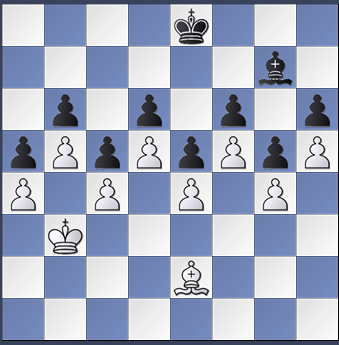
\includegraphics{exempledraw}

Aux yeux d'un joueur d'échec, cette partie est très clairement une égalité.
Cependant, il est très complexe pour un algorithme de le reconnaître.
Nous ne pouvons donc pas mettre en place toutes les possibilités différentes.

Notre gestion de la nulle est donc assez basique, nous ne vérifions que 2 cas particuliers.

Premièrement, nous vérifions la règle du pat : un des joueurs n'a aucun coup possible, mais il n'est pas en échec en mat.
Ensuite, on annonce nulle si un des deux rois à bougé plus de 30 fois d'affilé.
Enfin, à chaque tour, les joueurs peuvent conjointement décider de terminer sur un nul.
 
Voici l'implémentation des deux cas particuliers: 
\begin{minted}[mathescape,
    linenos,
    numbersep=5pt,
    gobble=2,
    frame=lines,
    framesep=2mm]{python}

    #PLACEHOLDER
\end{minted}


\subsubsection{Finalisation de la classe Piece}
Une fois l'EtatJeu mis en place, nous pouvons écrire la méthode coups légaux.

\begin{minted}[mathescape,
    linenos,
    numbersep=5pt,
    gobble=2,
    frame=lines,
    framesep=2mm]{python}

    #PLACEHOLDER
\end{minted}

\subsubsection{Classe Joueurs : Humain}
A ce stade, le noyau du jeu d'échecs est terminé. Pour le rendre jouable,
nous devons implémenter la classe Joueurs.
C'est la classe Joueurs qui sera, durant la partie, l'interface entre le programme main et les
classes Piece et EtatJeu, via la méthode jouer-coup.\\ En prévision de l'implémentation de l'IA,
on implémente une sous classe Humain, qui a sa propre méthode jouer-coup, car celle de l'IA sera différente.
Pour la classe Humain, la méthode jouer-coup doit interagir avec l'utilisateur. \\
On doit notamment effectuer la conversion des coordonnées du plateau en notation algébrique.


\begin{minted}[mathescape,
    linenos,
    numbersep=5pt,
    gobble=2,
    frame=lines,
    framesep=2mm]{python}

    #PLACEHOLDER
\end{minted}


\subsection{Le Programme main}
Au final, le jeu doit se joueur depuis un simple script main, qui utilise nos classes
définies dans des fichiers annexes.
Nous avons décidé d'implémenter ce programme avant de concevoir l'IA, 
afin de faciliter les tests.
On définit alors une fonction partie, qui créee (à partir des choix de l'utilisateur) et fait jouer une partie à l'utilisateur.
On place ensuite cette fonction dans une boucle, en demandant à l'utilisateur si il veut rejouer
à chaque fin de partie.
\begin{minted}[mathescape,
    linenos,
    numbersep=5pt,
    gobble=2,
    frame=lines,
    framesep=2mm]{python}

    #PLACEHOLDER
\end{minted}
\subsection{IA}
A FAIRE
\begin{minted}[mathescape,
    linenos,
    numbersep=5pt,
    gobble=2,
    frame=lines,
    framesep=2mm]{python}

    #PLACEHOLDER
\end{minted}

\section{Tests}
\section{peut être un de plus jsp}
\end{document}